% Copyright 2004 by Till Tantau <tantau@users.sourceforge.net>.
%
% In principle, this file can be redistributed and/or modified under
% the terms of the GNU Public License, version 2.
%
% However, this file is supposed to be a template to be modified
% for your own needs. For this reason, if you use this file as a
% template and not specifically distribute it as part of a another
% package/program, I grant the extra permission to freely copy and
% modify this file as you see fit and even to delete this copyright
% notice. 

\documentclass{beamer}

\usepackage{docmute}
\usepackage{pgfgantt}

\usepackage[utf8]{inputenc}
\usepackage[hungarian]{babel}
\usepackage{amsmath}

% There are many different themes available for Beamer. A comprehensive
% list with examples is given here:
% http://deic.uab.es/~iblanes/beamer_gallery/index_by_theme.html
% You can uncomment the themes below if you would like to use a different
% one:

\usetheme{Hannover}

\title{Unslaneta}
\subtitle{Statisztikus gépi fordítás}

\author{Bordi Eszter, Pável Szabolcs, Sándor Csanád}
% - Give the names in the same order as the appear in the paper.
% - Use the \inst{?} command only if the authors have different
%   affiliation.

\institute[Babe\c{s}-Bolyai Tudományegyetem] % (optional, but mostly needed)
{Babe\c{s}-Bolyai Tudományegyetem, Matematika és Informatika Kar, Kolozsvár}
% - Use the \inst command only if there are several affiliations.
% - Keep it simple, no one is interested in your street address.

\date{2016. június 23.}
% - Either use conference name or its abbreviation.
% - Not really informative to the audience, more for people (including
%   yourself) who are reading the slides online 

% If you have a file called "university-logo-filename.xxx", where xxx
% is a graphic format that can be processed by latex or pdflatex,
% resp., then you can add a logo as follows:

% \pgfdeclareimage[height=0.5cm]{university-logo}{university-logo-filename}
% \logo{\pgfuseimage{university-logo}}

% Let's get started
\begin{document}
\begin{frame}
  \titlepage
\end{frame}
\begin{frame}{Tartalom}
  \tableofcontents
  % You might wish to add the option [pausesections]
\end{frame}

% Sections are stored in separate .tex files

\section[Bevezető]{A statisztikus gépi fordítás  elméleti alapjai}
\begin{frame}{A statisztikus gépi fordítás alapjai}
  \begin{figure}[t]
  	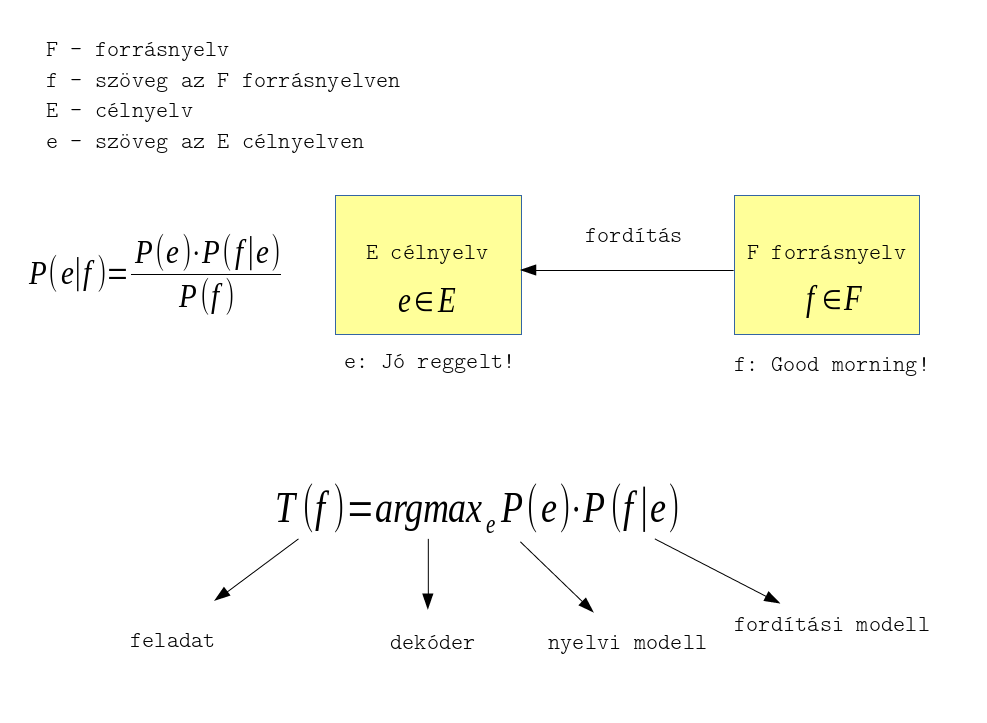
\includegraphics[width=1\linewidth]{images/smt}
  \end{figure}
\end{frame}

\begin{frame}{A statisztikus gépi fordítás alapjai}
  \begin{figure}[t]
  	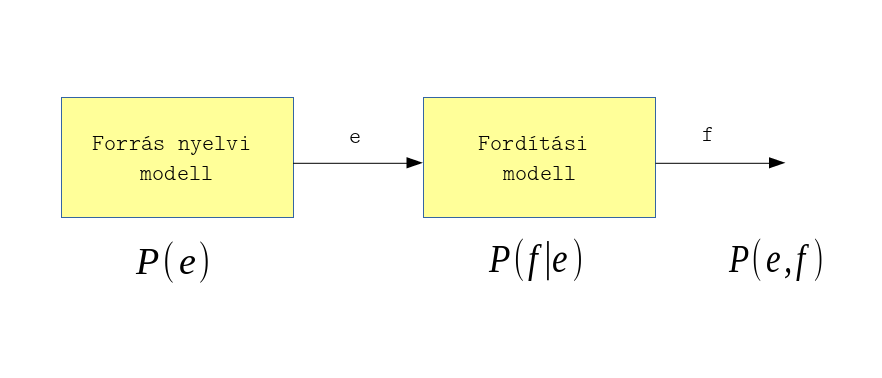
\includegraphics[width=1\linewidth]{images/smt2}
  \end{figure}
  
  \begin{itemize}
  	\item $P(e)$ nyelvi modell: n-gram modell
  	\item $P(f|e)$ fordítási modell: IBM modell
  	\item dekóder: StackDecoder
  \end{itemize}
\end{frame}

\begin{frame}{A nyelvi modell: bigrammok}
	\begin{itemize}
		\item Adva van egy angol szósorozat: $W = w_1,w_2,...,w_n$
		\item Lánc-szabály szerint: \begin{equation*}
		\begin{split}
		p(W) = p(w_1,w_2,...,w_n) = p(w_1) \cdot p(w_2|w_1) \cdot \\p(w_3|w_1, w_2) \cdot ... \cdot p(w_n|w_1,...,w_{n-1})
		\end{split}
		\end{equation*}
		\item \textbf{Markov-feltétel} bevezetése: a múlt legutolsó lépése számít
		\begin{equation*}
		\begin{split}
		p(w_1,w_2,...,w_n) = p(w_1) \cdot p(w_2|w_1) \cdot \\p(w_3|w_2) \cdot ... \cdot p(w_n|w_{n-1})
		\end{split}
		\end{equation*}
		\item ML-becslés: 
		\begin{equation*}
		p(w_2|w_1) = \frac{count(w_1,w_2)}{count(w_1)}
		\end{equation*}
	\end{itemize}
\end{frame}

\begin{frame}{IBM1 modell}
	\begin{itemize}
		\item \textbf{Kérdés}: Hogyan modellezük a $P(f|e)$ valószínűséget?
			\begin{equation*}
			\begin{split}
			f = f_1f_2...f_m\\
			e = e_1e_2...e_l
			\end{split}
			\end{equation*}
		\item m-et rögzítve kapjuk: $p(f_1f_2...f_m|e_1e_2...e_l, m)$
		\item Hozzávesszük még a célmondat szavainak lehetséges elrendezéseit:
		$p(f_1f_2...f_m, a_1...a_m|e_1e_2...e_l, m)$
		\item \textbf{Példa:}\\
				f = Le programme a ete mis en application\\
				e = And the programme has been implemented \\
				a = 0-1 1-2 2-3 3-4 4-5 5-5 5-5
	\end{itemize}

\end{frame}

\begin{frame}{IBM2 modell}
	\begin{figure}[t]
	  	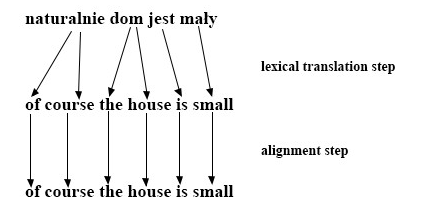
\includegraphics[width=1\linewidth]{images/ibm2}
	  	\caption{IBM2 modell\footnotemark}
	  \end{figure}
\footnotetext{\href{https://en.wikipedia.org/wiki/IBM_alignment_models}{Forrás IBM2 modell}}
\end{frame}

\section[Megvalósítás]{Mit használtunk fel?}




% Section and subsections will appear in the presentation overview
% and table of contents.
%\section{First Main Section}
%
%\subsection{First Subsection}
%
%\begin{frame}{First Slide Title}{Optional Subtitle}
%  \begin{itemize}
%  \item {
%    My first point.
%  }
%  \item {
%    My second point.
%  }
%  \end{itemize}
%\end{frame}
%
%\subsection{Second Subsection}
%
%% You can reveal the parts of a slide one at a time
%% with the \pause command:
%\begin{frame}{Second Slide Title}
%  \begin{itemize}
%  \item {
%    First item.
%    \pause % The slide will pause after showing the first item
%  }
%  \item {   
%    Second item.
%  }
%  % You can also specify when the content should appear
%  % by using <n->:
%  \item<3-> {
%    Third item.
%  }
%  \item<4-> {
%    Fourth item.
%  }
%  % or you can use the \uncover command to reveal general
%  % content (not just \items):
%  \item<5-> {
%    Fifth item. \uncover<6->{Extra text in the fifth item.}
%  }
%  \end{itemize}
%\end{frame}
%
%\section{Second Main Section}
%
%\subsection{Another Subsection}
%
%\begin{frame}{Blocks}
%\begin{block}{Block Title}
%You can also highlight sections of your presentation in a block, with it's own title
%\end{block}
%\begin{theorem}
%There are separate environments for theorems, examples, definitions and proofs.
%\end{theorem}
%\begin{example}
%Here is an example of an example block.
%\end{example}
%\end{frame}
%
%% Placing a * after \section means it will not show in the
%% outline or table of contents.
%\section*{Summary}
%
%\begin{frame}{Summary}
%  \begin{itemize}
%  \item
%    The \alert{first main message} of your talk in one or two lines.
%  \item
%    The \alert{second main message} of your talk in one or two lines.
%  \item
%    Perhaps a \alert{third message}, but not more than that.
%  \end{itemize}
%  
%  \begin{itemize}
%  \item
%    Outlook
%    \begin{itemize}
%    \item
%      Something you haven't solved.
%    \item
%      Something else you haven't solved.
%    \end{itemize}
%  \end{itemize}
%\end{frame}



% All of the following is optional and typically not needed. 
\appendix
\section<presentation>*{\appendixname}
\subsection<presentation>*{Irodalomjegyzék}


\begin{frame}[allowframebreaks]
        \frametitle{Irodalomjegyzék}
        \bibliographystyle{amsalpha}
        \bibliography{referencia}
\end{frame}

\end{document}


